\chapter{Refraktionsseismik}
In diesem Kapitel beschäftigen wir uns mit refraktierten seismischen Wellen. Diese Wellen laufen entlang der Schichtgrenze und strahlen konstant neue Wellen unter dem kritischen Winkel zurück zur Erdoberfläche. Eine solche Welle tritt auf, wenn eine seismische Welle unter dem kritischen Winkel auf die Schichtgrenze trifft. Weiterhin muss dabei die Geschwindigkeit nach unten hin zunehmen. Die refraktierte Welle wird im Allgemeinen auch als \textbf{Kopfwelle} bezeichnet. 

Durch einen Hammerschlag, eine kleine Explosion oder andere Quellen werden an der Oberfläche oder wenige Meter im Erdinnern künstlich seismische Wellen erzeugt. Deren Ausbreitung wird an der Oberfläche mit Hilfe von Geophonen aufgezeichnet. Diese Sensoren sind entlang einer festen Linie (\textbf{Profillinie}) in gleichmäßigem Abstand ausgelegt. Die Abstände zwischen den Messgeräten können wenige Meter bis mehrere Kilometer betragen. Die Gesamtlänge der Profillinie ist zwischen einige zehn Meter bis mehr als 100 Kilometer lang, je nach gewünschter Tiefe der Untersuchung. 

Aus den gemessenen Daten wird ein \textbf{Laufzeitdiagramm} erstellt und ausgewertet. Dabei wird besonders die refraktierte Welle betrachtet. Das Ergebnis dieser Auswertung ist ein Untergrundmodell, welches die einzelnen Schichten mit ihrer jeweiligen Wellengeschwindigkeit zeigt.  

Anwendung finden refraktionsseismische Verfahren beispielsweise in geologischen Erkundungen der Erdkruste und des oberen Erdmantels, wie z.B. die Ermittlung der Tiefe einer Gebirgswurzel.   

\section{Der söhlige Zweischichtfall}
Um die refraktionsseismischen Verfahren zu verstehen, beginnen wir mit dem einfachsten Fall. Der zu untersuchende Untergrund hat eine Schichtgrenze, die horizontal (\textbf{söhlig}) verläuft. Unser Ziel dabei ist die Berechnung der Tiefe der Schichtgrenze (\textbf{Mächtigkeit}) und die Ausbreitungsgeschwindigkeiten in beiden Schichten.

\subsection{Strahlenwege und Laufzeitgleichungen}
Zu Beginn betrachten wir einmal den Verlauf der Wellenstrahlen im Untergrund und deren Laufzeitgleichungen. Letztere lassen sich durch einfache geometrische Überlegungen herleiten. 

\begin{figure}[H]
	\centering
	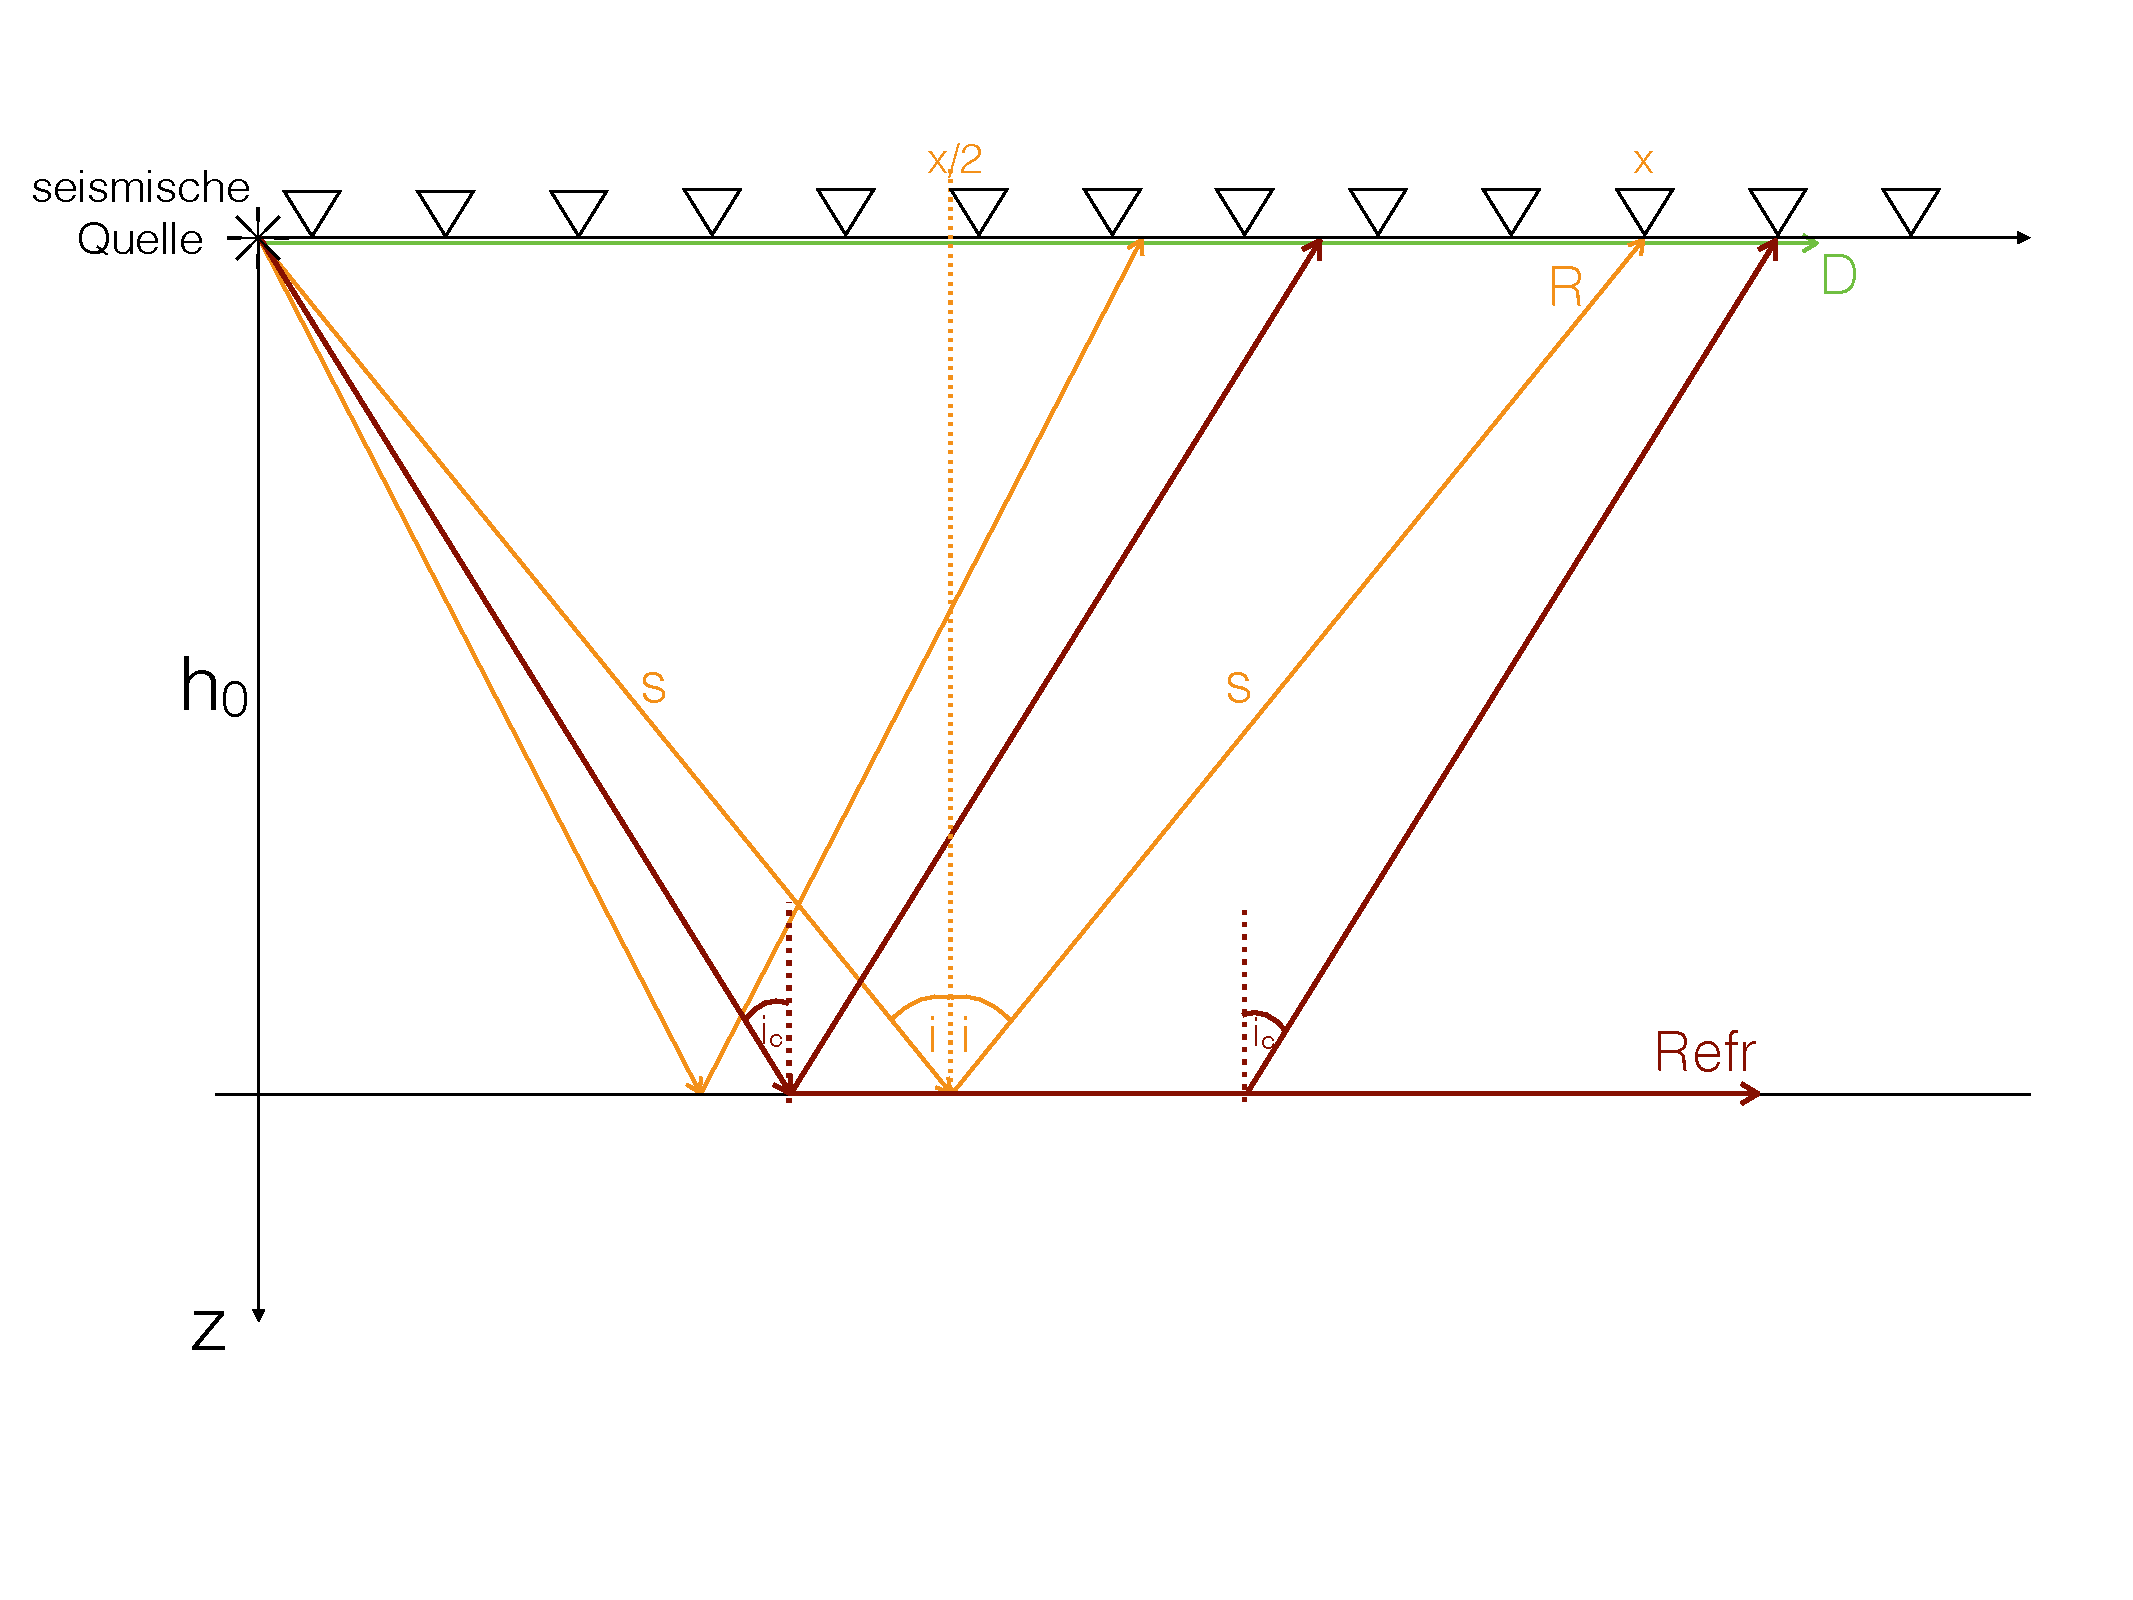
\includegraphics[width = \textwidth]{RefraktionsseismikBilder/soehliger2SchichtFallStrahlen}
\end{figure}


\subsubsection{Direkte Welle (D)}
Diese Welle bewegt sich mit konstanter Geschwindigkeit direkt unter der Erdoberfläche fort. Die Zeit bis zum Antreffen an Punkt $x$ berechnet sich so: \begin{equation*}
	t_{\text{D}} = \frac{x}{v_0}
\end{equation*}

\subsubsection{Reflektierte Welle (R)}
Die Wellenstrahlen werden an der Grenzfläche reflektiert. Es gilt "`Einfallswinkel = Ausfallswinkel"'. Ihre Laufzeit lässt sich folgendermaßen berechnen: \begin{equation*}
	t_{\text{R}} = \frac{2 \cdot s}{v_0} = \frac{2 \cdot \sqrt{\left( \frac{x}{2} \right) ^2 + h_0^2}}{v_0}
\end{equation*}
Um den Wurzelterm zu vereinfachen, quadriert man die gesamte Gleichung: \begin{equation*}
	t_{\text{R}}^2 = \left( \frac{x}{v_0} \right)^2 + \left( \frac{2 \cdot h_0}{v_0} \right) ^2 =  \left( \frac{x}{v_0} \right)^2 + t_0^2
\end{equation*}
Wobei $t_0$ der Ersteinsatz der reflektierten Welle ist.

\subsubsection{Refraktierte Welle (Refr)}
Die Wellenstrahlen treffen unter dem kritischen Winkel auf die Grenzfläche und verlaufen entlang dieser. Dabei werden kontinuierlich neue Wellenstrahlen unter dem kritischen Winkel zur Erdoberfläche zurück gestrahlt. Die Laufzeit der refraktierten Welle berechnet sich so: \begin{equation*}
	t_{\text{Refr}} = \frac{2 \cdot h_0 \cdot cos(i_c)}{v_0} + \frac{x}{v_1}
\end{equation*}



\subsection{Laufzeitdiagramm}
Die Ergebnisse unserer Messung übertragen wir in ein Diagramm. 

\begin{figure}[H]
	\centering
	\includegraphics[width = \textwidth]{RefraktionsseismikBilder/LaufzeitdiagrammSöhlig}
\end{figure}

Es seinen noch einige Begriffe aus dem Diagramm erklärt: \begin{description}
	\item[kritische Entfernung $x_{\text{c}}$:] Bei dieser Entfernung tritt die refraktierte Welle das erste Mal auf, d.h. sie wird das erste Mal von einem Geophon gemessen. 
	\item[Knickpunkt $x_{\text{k}}$:] An diesem Punkt überholt die refraktierte Welle die direkte Welle.
	\item[Interceptzeit $t_{\text{i}}$:] Diese Zeit bezeichnet den errechneten, theoretischen Ersteinsatz der Kopfwelle.  
\end{description}

\subsection{Auswertung}
Wie bereits erwähnt, interessieren uns die Ausbreitungsgeschwindigkeiten $v_0$ und $v_1$ der Schichten, sowie die Tiefe $h_0$ der Schichtgrenze.

\subsubsection{Wellengeschwindigkeit $v_0$}
Die Ausbreitungsgeschwindigkeit einer seismischen Welle in der oberen Schicht ergibt sich direkt aus der Steigung der direkten Welle: \begin{equation*}
	v_0 = \frac{x}{t_{\text{D}}}
\end{equation*}

\subsubsection{Wellengeschwindigkeit $v_1$}
Die Geschwindigkeit der zweiten Schicht ergibt sich auch sehr einfach aus der Steigung der refraktierten Welle: \begin{equation*}
	v_1 = \frac{\Delta x}{\Delta t_{\text{refr}}}
\end{equation*}

\subsubsection{Schichtmächtigkeit $h_0$: Möglichkeit 1}
Ein Ansatz zur Berechnung von $h_0$ ergibt sich aus der Intercept-Zeit: \begin{equation*}
	t_i = \frac{2 \cdot h_0 \cdot cos(i_c)}{v_0}
\end{equation*}
Diese Gleichung stellen wir nach $h_0$ um: \begin{equation*}
	h_0 = \frac{v_0 \cdot t_{\text{i}}}{2 \cdot cos(i_c)}
\end{equation*}
Wir möchten nun noch den kritischen Winkel in der Gleichung ersetzen. Hierzu verwenden wir den mathematischen Zusammenhang: \begin{equation*}
	cos(i_c) = \sqrt{1 - sin^2(i_c)} 
\end{equation*} 
Weiterhin wissen wir, wie sich der kritische Winkel mit dem Sinus ausdrücken lässt. \begin{equation*}
	sin(i_c) = \frac{v_0}{v_1}
\end{equation*}
Hieraus ergibt sich dann die Formel zur Berechnung von $h_0$: \begin{equation*}
	h_0 = \frac{t_{\text{i}}}{2} \cdot \frac{v_0 \cdot v_1}{\sqrt{v_1^2 - v_0^2}}
\end{equation*}


\subsubsection{Schichtmächtigkeit $h_0$: Möglichkeit 2}
Eine weitere Möglichkeit ist die Berechnung mit Hilfe des Knickpunktes. An dieser Stelle sind die Laufzeit von direkter Welle und refraktierter Welle gleich, also setzen wir die Laufzeitgleichungen gleich: \begin{equation*}
	t_{\text{D}}(x_{\text{k}}) = t_{\text{Refr}}(x_{\text{k}}) \quad \Rightarrow \quad h_0 = \frac{x_{\text{k}}}{2} \cdot \sqrt{\frac{v_1 - v_0}{v_1 + v_0}}
\end{equation*}


\subsubsection{Schichtmächtigkeit $h_0$: Möglichkeit 3}
Die letzte Variante ist die Berechnung aus der $t_0$-Zeit. Die Formel hierfür ergibt sich direkt durch Umstellen: \begin{equation*}
	h_0 = \frac{v_0 \cdot t_0}{2}
\end{equation*}



\section{Der geneigte Zweischichtfall}
Dass die Schichtgrenze exakt horizontal verläuft, ist ein sehr unwahrscheinlicher Fall. In der Regel ist die Schichtgrenze um einen Winkel $\delta$ geneigt. Damit sich die Schichtgeschwindigkeiten dennoch berechnen lassen, werden zwei Messungen durchgeführt. Die eine Messung beginnt an einem Ende der Profillinie, die Zweite am anderen Ende. Erstere Messung nennt man \textbf{Hinschuss} und die zweite Messung entsprechend \textbf{Rückschuss}. Der kritische Winkel der Welle verändert sich durch die Schichtneigung nicht.

\subsection{Strahlenwege}
Auch hier wollen wir uns zunächst einmal den Verlauf der Wellen anschauen. Um die Grafik etwas übersichtlicher zu gestalten, tragen wir nur den Verlauf der Strahlen der refraktierten Welle von Hin- und Rückschuss ein.

\begin{figure}[H]
	\centering
	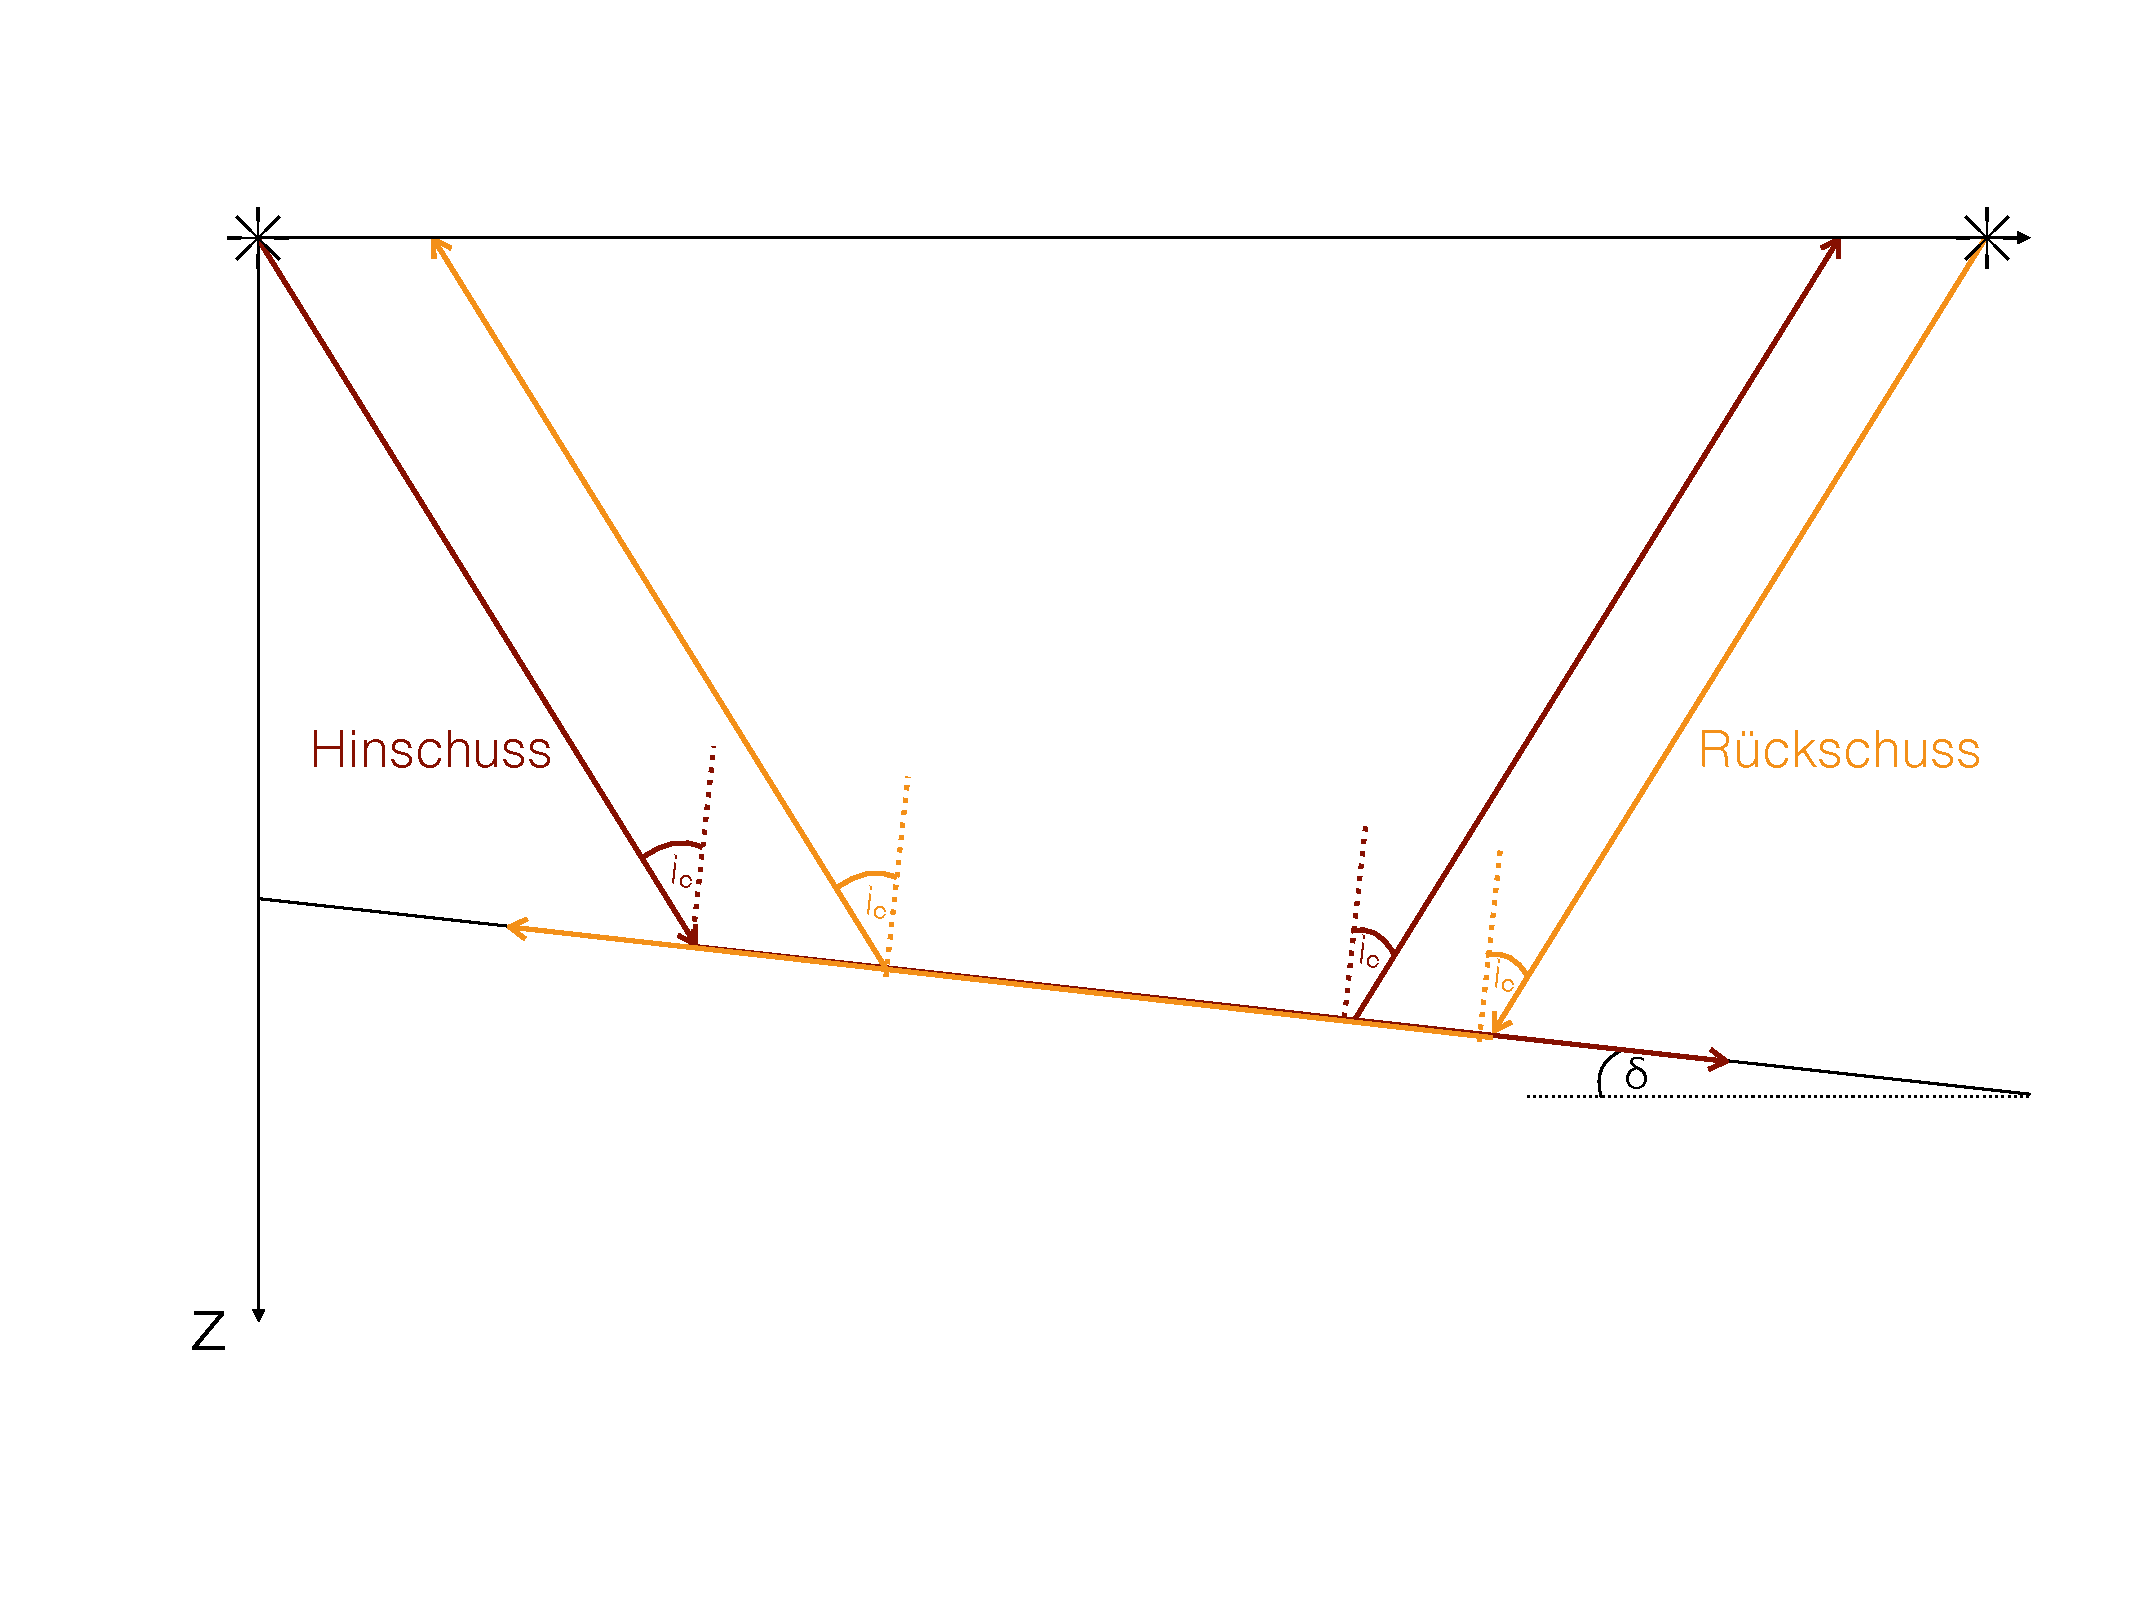
\includegraphics[width = \textwidth]{RefraktionsseismikBilder/geneigteSchichtStrahlen}
\end{figure}


\subsection{Laufzeitdiagramm}
Auch hier übertragen wir die Messergebnisse in ein Diagramm. 

\begin{figure}[H]
	\centering
	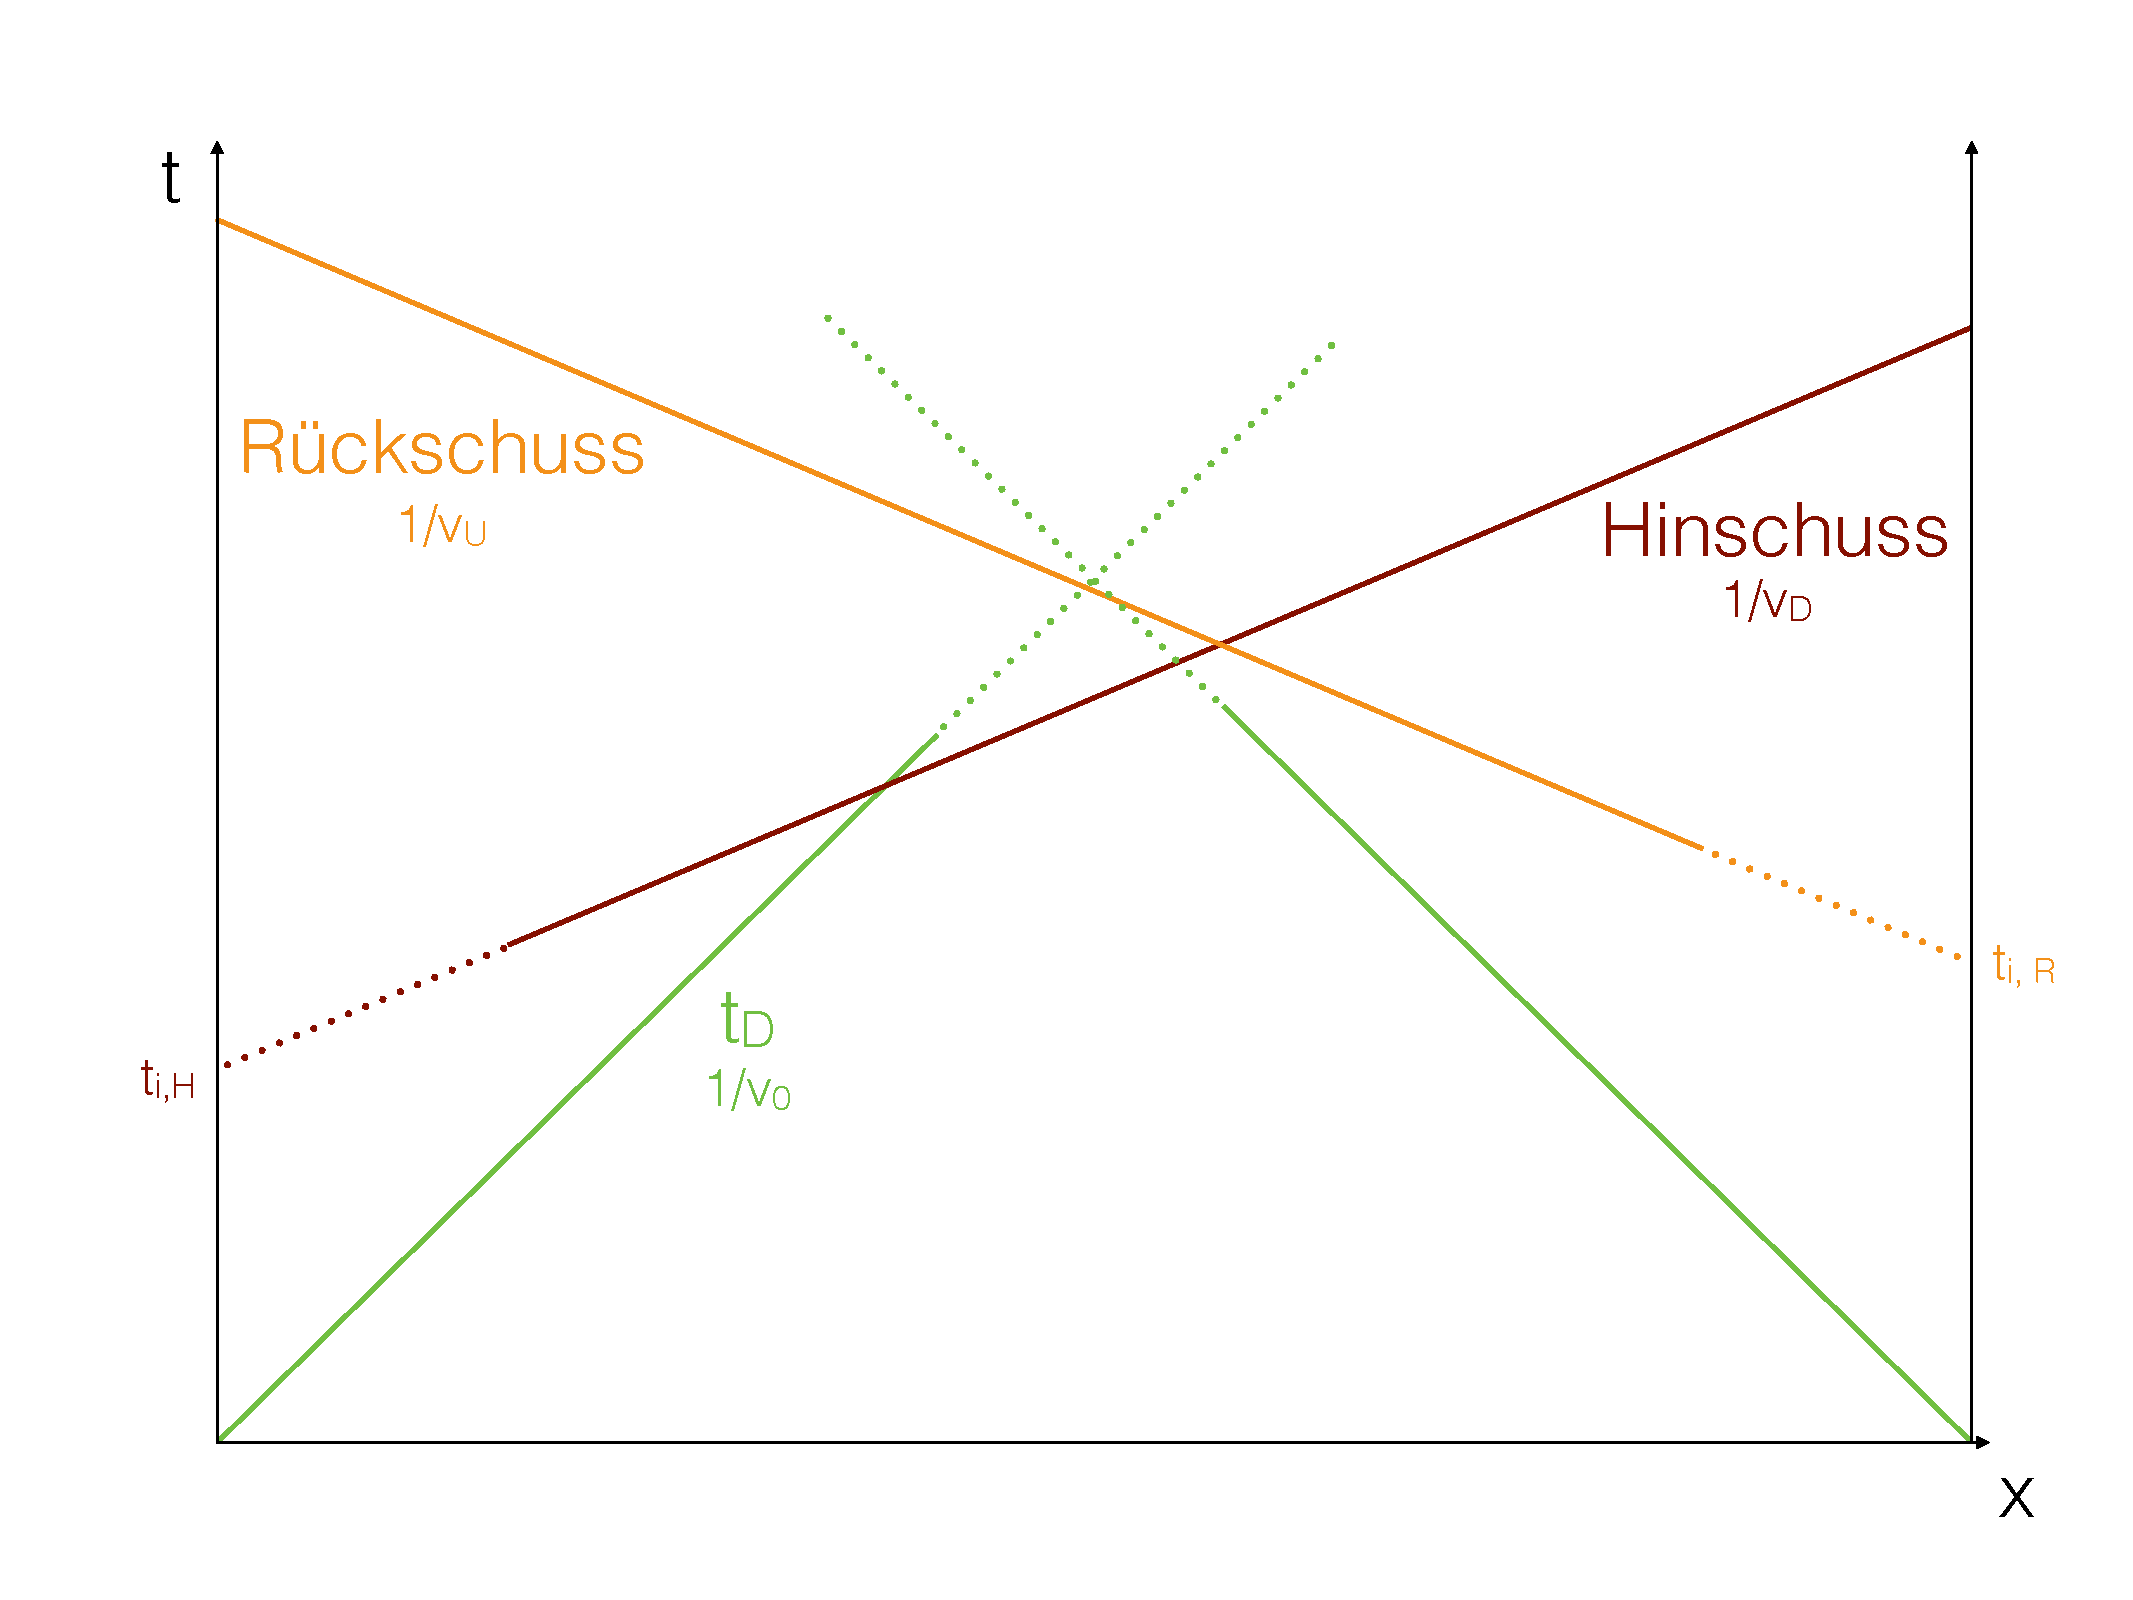
\includegraphics[width = \textwidth]{RefraktionsseismikBilder/LaufzeitdiagrammGeneigt}
\end{figure}

In dieser Grafik haben wir die Wellengeschwindigkeit beim Hinschuss $v_{\text{D}}$ und beim Rückschuss $v_{\text{U}}$ genannt. D und U stehen dabei für "`Down-Dip"' bzw. "`Up-Dip"' Geschwindigkeit. 

Wir benutzen die Steigungen der refraktierten Wellen von Hin- und Rückschuss, um die Schichtgeschwindigkeiten zu berechnen. Im Folgenden sei $v_0$ die Wellengeschwindigkeit in der oberen Schicht und $v_1$ die Geschwindigkeit in der Schicht unter der geneigten Grenzfläche. 

$v_0$ ergibt sich direkt durch Umstellen der Steigungsgleichungen von Up- und Down-Dip: \begin{align*}
		\frac{1}{v_{\text{U}}} &= \frac{sin(i_c - \delta)}{v_0} \\
		\frac{1}{v_{\text{D}}} &= \frac{sin(i_c + \delta)}{v_0}
\end{align*}

$v_1$ ergibt sich wiederum einfach durch den kritischen Winkel: \begin{equation*}
	\frac{1}{v_1} = \frac{sin(i_c)}{v_0}
\end{equation*}

Um $v_0$ hierfür nicht extra berechnen zu müssen, aproximieren wir die Gleichung und drücken sie durch $v_{\text{D}}$ und $v_{\text{U}}$ aus: \begin{equation*}
	\frac{1}{v_1} = \frac{sin(i_c)}{v_0} \approx \frac{sin(i_c + \delta) + sin(i_c - \delta)}{2 v_0} = \frac{1}{2} \left( \frac{1}{v_{\text{U}}} + \frac{1}{v_{\text{D}}} \right)
\end{equation*}




